%Report
\documentclass[14pt]{extreport}
\usepackage{color}
\usepackage[cache=false]{minted}
\usepackage{afterpage}
\usepackage{graphicx}
\usepackage[backend=biber]{biblatex}
\usepackage[utf8]{inputenc}
\usepackage{hyperref}

\bibliography{refs.bib}

% Command for inserting blank page
\newcommand\blankpage{
    \null
    \thispagestyle{empty}
    %\addtocounter{page}{-1}
    \newpage
    }

\title{High Performance Graph Processing in Partitioned Global Address Space Model}
\date{2020--12--10}
\author{Vahag Bejanyan}

\begin{document}

\maketitle
\pagenumbering{gobble}
\newpage
\pagenumbering{arabic}

\tableofcontents
\blankpage

\chapter{Introduction}
Graphs are playing an emerging role in the field of Computer Science. Various problems can be modeled and studied as graphs\cite{fouss_saerens_shimbo_2016}. Hence, to be able to solve large graph problems effectively the fast, stable, and accurate algorithms, new computation models and frameworks are needed to express graph-based computations and simulations. Often graphs can reach up to hundreds of millions of vertices in size, hence simple serial implementations are not feasible for such cases. One of the possible ways to overcome these limitations is the use of shared memory models for parallel programming\cite{patterson_hennessy}. Using shared memory parallel programming it would be possible to explore the computational power of all the cores present on a chip rather than limiting computation in the scope of one core. On the other hand, when dealing with large data analytics problems\cite{hadoop}\cite{mapreduce}, volumes of the dataset can reach petabytes, and the need for cluster computing and huge memory storages arise.  One of the widely used and adopted models to express distributed computations is the Message Passing Interface(hereafter MPI) protocol. In essence, MPI provides a generic API through which various computation nodes can be grouped into communicator groups and exchange messages through both synchronous and asynchronous interfaces. Another important aspect of the distributed programming approach is the proper selection of a distributed memory management model\cite{dsmmng}. These models for the distributed shared memory management can either be centrilized or distributed and on their own distributed models are either fixed or dynamic. The model chose for the management of distributed shared memory can hugely affect the performance, energy consumption, and stability of the overall system. Partitioned Global Address Space(hereafter PGAS) models act as a new alternative for distributed scalable computing. In future sections of this document various PGAS powered models such as Chapel and UPC++ will be described. An overview of actual research related to PGAS powered graph algorithms and models will be given. Research objectives will be sited.

\blankpage
\chapter{Research objectives}
In the scope of the planned research following objectives are set:

\begin{enumerate}
	\item Research opportunities that PGAS powered computation models provide for HPC.
	\item Investigate Performance and Energy Efficiency of the distributed graph processing algorithms for the PGAS Programming Model for HPC Graph processing in comparison to MPI and MPI+PGAS
	\item Performance and Energy Efficiency evaluations of distributed graph processing algorithms for Chapel and PGAS.
	\item Study distributed graph algorithms in the PGAS model.
	\item A methods and SaaS Cloud Services for distributed graph processing algorithms.
	\item Study and develop PGAS powered frameworks for HPC, graph analysis, and graph-theoretic machine learning.
\end{enumerate}

\blankpage
\chapter{Background}
\section{Parallel Programming Models}
\subsection{Shared Memory Models}
This model is based on shared memory systems, where each memory location is accessible by every computation node. Usually, multithreaded programming models are implemented as a shared memory system. In this model, any memory location is globally accessible and control is synchronized through the usual synchronization primitives like mutexes. Many languages like C++11 provide an Abstract Memory Model which alongside its standardized threads support be used in shared memory system programming. Other examples are Pthreads and OpenMP which both provide API for multithreaded execution in shared memory systems.
\subsection{Distributed Memory Models}
In this model, each processor maintains, its own local memory and knows nothing about other computation units.
To be able to communicate in this model a message-passing protocol(like MPI) should be established. For distributed memory model computing MPI provides a rich set of features such as:
\begin{enumerate}
\item Point-to-point Two-sided Communication
\item Collective Communication 
\item One-Sided Communication
\item Job Startup
\item Parallel I/O
\end{enumerate}

\subsection{Partitioned Global Address Space}
Partitioned Global Address Space (PGAS) is a parallel programming model which assumes global view on address space which is partitioned within different processes. Below given a list of characteristics that language should specify to be considered as PGAS lanauge\cite{pgaslangs}.
\begin{enumerate}
	\item It should specify a parallel execution model,
	\item It should provide a way to specify how a global address space should be partitioned,
	\item It should provide a way to describe how data is distributed over different partitions,
	\item Language should allow access to both shared and distributed data using shared-memory semantics.
\end{enumerate}

\paragraph{Parallel Execution Model}
This model describes the details of launching and executing parallel activities(hereafter threads). PGAS model provides three main kinds of such activities.

\subparagraph{Single Program Multiple Data}
In this model at the program startup, a fixed number of threads is created. Each thread has its unique thread index and hence using this index, for example, it's possible to specify which data the current thread should process.

\subparagraph{Asynchronous PGAS}
In this model at the program startup, only one thread is created. Creation of new threads has dynamic fashion and expressed using language-specific constructs like \mintinline{chapel}{cobegin} in the case of Chapel.

\subparagraph{Impilicit Parallelism} In this model no explicit parallelism exists in code. Instead of that new thread creation is done by the language runtime and data distributed handled in an opaque way. Chapels \mintinline{chapel}{forall} construct is a good example of this concept.

\subparagraph{Places Model}
Large-scale systems with multiple computational nodes often incorporate NUMA characteristics. To cope with this, in the PGAS model global address space is partitioned into so-called \textit{places}. This differentiation allows to easily express an affinity of memory to its computation node. This allows the node to access memory at a minimal cost. On the other side, access to data from a different \textit{places} has a higher cost.

\subparagraph{Data Distribution Model}\label{DataDistributionModelSubParagraph}
This model describes how data is distributed over different places. Distributions can be regular and irregular. An example of a regular distribution is globally distributed partitioned arrays which Chapel provided. Before creating such an array an index set is specified which determines how data should be distributed over places(or \textit{Locales}) in case of Chapel). Several patterns are possible for regular distributions. For example (a) cyclic-distribution, (b) block-cyclic-distribution and (c) block-distribution are common.

\begin{figure}[H]
	\centering
	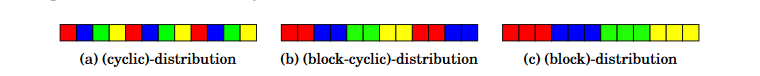
\includegraphics[scale=1]{images/distributions.png}
	\caption{Visualization of distributions}
\end{figure}

Below are given examples of how index set distribution can be expressed using Chapel.

\begin{listing}[H]
\begin{minted}[tabsize=4,linenos]{chapel}
// Make the program size configurable from the command line.
config const n = 8;

// Declare a 2-dimensional domain Space that we 
// will later use to initialize the distributed domains.
const Space = {1..n, 1..n};

// The Block distribution distributes a bounding 
// box from n-dimensional space across the target locale 
// array viewed as an n-dimensional virtual locale grid. 
// The bounding box is blocked into roughly equal 
// portions across the locales. 
// Note that domains declared over a Block distribution can also 
// store indices outside of the bounding box;
// the bounding box is merely used to compute the blocking of space.
const BlockSpace = Space dmapped Block(boundingBox=Space);
var BA: [BlockSpace] int;

// Cyclic distributions start at a designated n-dimensional 
// index and distribute the n-dimensional space across 
// an n-dimensional array of locales in 
// a round-robin fashion (in each dimension).
const CyclicSpace = Space dmapped Cyclic(startIdx=Space.low);
var CA: [CyclicSpace] int;

// Block-Cyclic distributions also deal out indices in a 
// round-robin fashion, but rather than dealing out 
// singleton indices, they deal out blocks of indices. 
// Thus, the BlockCyclic distribution is parameterized by 
// a starting index (as with Cyclic) and a block 
// size (per dimension) specifying how large the 
// chunks to be dealt out are.
const BlkCycSpace = Space dmapped BlockCyclic(startIdx=Space.low,
                                              blocksize=(2, 3));
var BCA: [BlkCycSpace] int;
\end{minted}
\caption{Examples of Index Distributions in Chapel}
\label{ChapelExamples}
\end{listing}

On the other side, irregular distribution can play a significant role in a construction of irregular data structures such as trees or hashmaps. To achieve this UPC++\cite{upcpp} achieves this in terms for \textit{Global Pointers}, \textit{futures} and \textit{distributed objects}. UPC++ also leverages \textit{1-sided communication}, which can lead to better performance because of lock constraints on package ordering and \textit{RPC}. UPC++ provides several ways for synchronizing activities, namely \textit{barriers} and \textit{asynchronous barriers} which are used in couple with futures. Below given an example implementation of distributed hashmap using UPC++ and C++.

\begin{listing}[H]
\begin{minted}[tabsize=4,linenos]{c++}
class DistrMap {
	using dobj_map_t = upcxx::dist_object<
								std::unordered_map<std::string,	
												   std::string>>;
	dobj_map_t local_map;

	int get_target_rank(const std::string& key) {
		return std::hash<std::string>{}(key) % upcxx::rank_n();
	}

	public:
	DistrMap() : local_map({}) {}

	upcxx::future<> insert(const std::string& key, 
						   const std::string& val) {
		return upcxx::rpc(get_target_rank(key),
				[](dobj_map_t& lmap, 
				   const std::string& key, 
				   const std::string& val) {
				lmap->insert({key, val});
				}, local_map, key, val);
	}

	upcxx::future<std::string> find(const std::string& key) {
		return upcxx::rpc(get_target_rank(key),
				[](dobj_map_t& lmap, 
				   const std::string& key) -> std::string {
				auto elem = lmap->find(key);
				if (elem == lmap->end()) return std::string();
				return elem->second;
				}, local_map, key);
	}
};
\end{minted}
\caption{Distributed Hash Table using UPC++ Global Pointers}
\end{listing}

However, current PGAS models don't provide any standard irregular distributions like in the case of regular ones in this should be done explicitly by sharing pointers.

\subparagraph{Data Access Model}
This model is tightly connected to the \ref{DataDistributionModelSubParagraph} as it describes how data is distributed across places, represented, declared, and accessed. For example, in the case of regular distributions, a concept of local and global indexes is presented. Also, a distinction in global data access syntax is present, then such access is called explicit.

\blankpage
\chapter{Related Work}
The research was done to investigate results that already present in the area of PGAS powered models, and particularly, in the area of graph algorithms and analysis. In the rest of this section, several articles and projects that are in the area of interest will be described.
\section{Chapel Programming Language}
One of the projects that are being actively developed and are in the area of interest is a Chapel, a Productive Parallel Programming Language. Chapel inherits and implements many of the characteristics of the PGAS model described above. Chapel provides many built-in language features and modules that are simplifying parallel and distributed computing. A good example of such functionality are \textit{domains} and \textit{distributions}.
\paragraph{Domains}\label{DomainsSubParagraph}
From Chapel's documentation, it's known that domain is a first-class representation of an index set used to specify iteration spaces, define arrays, and aggregate operations, such as slicing. Domains can be rectangular and multidimensional and thus each dimension can be specified in terms of ranges. For example, to specify a 3D dimensional domain with equal dimensions, the Chapel provides the following syntax:

\begin{listing}[H]
\begin{minted}[tabsize=4,linenos]{chapel}
config var n = 10;
var RD: domain(3) = {1..n, 1..n, 1..n};
\end{minted}
\caption{Chapel Domains}
\end{listing}

Also Chapel provides support for the \textit{sparse} domains. They are usually stored in a Compressed Sparse Row(CSR) format. Support for this kind of features in a combination with its reach support for parallel and distributed computing makes a Chapel a very interesting candidate for numerical algorithms, simulations, and analysis of sparse graphs.

\paragraph{Distributions} Distributions are usually used in a combination with \ref{DomainsSubParagraph}. They are used to describe how a domain is distributed over the computing grid.
Chapel comes with a reach set of standard distributions, such as:

\begin{enumerate}
	\item BlockDist
	\item CyclicDist
	\item BlockCycDist
	\item DimensionalDist2D
	\item BlockCycDim
	\item ReplicatedDim
\end{enumerate}

Examples use cases for these are provided in the listing \ref{ChapelExamples}. The chapel also provides support for replicated distributions. The main difference from the other distributions is that this one stores all domain indices per local, by default, targeting all locales. And similarly, an array declared over a domain with such distribution will store copies of all its items per local. Such an array is called replicated and each locale's copy of such array or domain is called replicand.

\section{UPC++}
UPC++\cite{upcpp} presents itself as an PGAS extension for C++. UPC++ is implemented in a "compiler-free" approach as a library with reach use of C++ templates. This approach has several advantages, in particular, it allows compilers such as Clang or GCC to perform reach optimizations that they support and at the same time don't depend on data dependencies.
UPC++ incorporates the SPMD approach, described in previous sections. A unit of execution in UPC++ is called \textit{thread} and can be implemented in terms of OS-level threads or Pthreads. As UPC++ is SPMD powered, that number of threads is fixed at execution time.
UPC++ provides \textit{shared} type qualifiers to mark a scalar or array as shared. In the case of an array, they are implicitly shared in a block-cyclic fashion and such flexibility as with Chapel programs is not present here. Also UPC++ provides \textit{global pointers} to point to the shared memory locations. In a global address space model that this framework provides, each thread has associated with two kinds of address segments \textit{private} and \textit{shared}. This is illustrated in the figure below:
\begin{figure}[H]
	\centering
	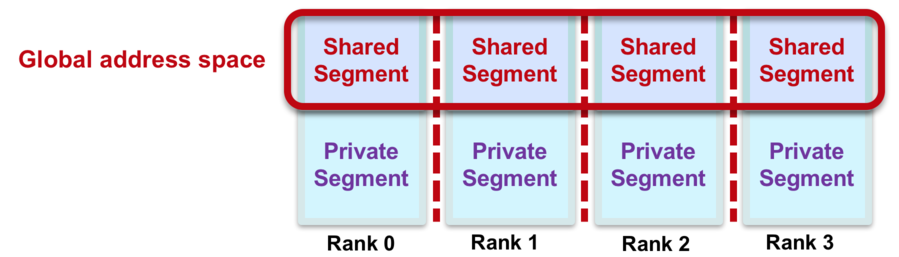
\includegraphics[scale=0.75]{images/global_address_space.png}
	\caption{Global Address Space Model}
\end{figure}

\section{Chapel Hypergraph Library}
The Chapel Hypergraph Library provides a Chapel implementation of abstractions to work with hypergraphs and several algorithms implemented in the PGAS model. In related research \cite{chgl} authors present an experimental evaluation of three hypergraph generation algorithms, namely:

\begin{enumerate}
	\item Hypergraph Erdos-Renyi (ER)
	\item Hypergraph Chung-Lu (CL)
	\item Hypergraph Block-Two Level Erdos-Renyi (BTER)
\end{enumerate}

For example, benchmarks of (ER) on the shared-memory model show a linear scaling when the number of cores is increasing by a power of two. On the opposite side, in distributed memory benchmark execution time increases because of constant communication time introduced into the program.

\section{Arkouda}
Arkouda\cite{arkouda} is another good example of a scientific computing library for Chapel. The core part of an Arkouda is constructed as a compact, highly scalable Chapel interpreter. This interpreter implements a powerful set of data science primitives. Interpreter consists of the dispatcher, modular data transformations, and zero-copy, in-memory object-store. In some sense, Arkouda tries to implement NumPy like libraries in Chapel for massive HPC.

\section{BCL}
BCL\cite{bcl} is a cross-platform distributed container library written in C++ using UPC++. The main aim of this library is to provide a set of generic, reusable high-performance \textit{irregular} data structures. BCL tries to fill that gap in libraries that are backed by MPI or PGAS and implemented their support using one-sided communication. Additionally, BCL can be backed by GASNet-EX, OpenSHMEM, UPC++. 

\section{GraphBLAS and Chapel}
Basic Linear Algebra Subprograms(BLAS)\cite{blas} is a collection of highly optimized primitives, building blocks for operations on vectors and matrices. GraphBLAS\cite{graphblasmath} is a project whose aim is to express graph algorithms using concepts from linear algebra and linear algebraic operations. In \cite{graphlinalg} necessary background in this field and basic graph algorithms based on linear algebra operations are expressed. In another research, \cite{azadb17a} a detailed discussion and analysis of possible GraphBLAS API Chapel implementation are given.

\printbibliography

\end{document}
